\documentclass[]{myclass}
\usepackage[cp1250]{inputenc}
\usepackage[OT4]{fontenc}
\usepackage{hyperref}
\usepackage[table,xcdraw]{xcolor}
\usepackage{multirow}
\usepackage{subfig}
\usepackage{float}
\usepackage{amsfonts}
\usepackage{pdfpages}
\usepackage{listings}
\usepackage[english]{babel}
\usepackage{titling}
\usepackage{tocbibind}
\usepackage[all]{nowidow}
\usepackage{comment}
\definecolor{mygreen}{rgb}{0,0.6,0}
\lstset {
basicstyle=\small,
breaklines=true,
commentstyle=\color{mygreen},
keywordstyle=\color{blue},
language=C,
linewidth=\textwidth
}
\linespread{1}

\author{Marcin Aftowicz}
\title{Hardware Test and fault diagnosis based on extended FEC functions  in wireless communication systems}
\mysupervisor{Prof. Dr.-Ing. H. T. Vierhaus \and Ing. Petr Pfeifer, MSc, MBA, Ph.D.}
\myyear{2018}

\begin{document}
\selectlanguage{english}
\bibliographystyle{plplain}

% Front matter **************************************
\frontmatter
\pagestyle{empty}%
\maketitle  \cleardoublepage

\pagenumbering{Roman}
\phantomsection
\addcontentsline{toc}{chapter}{Statutory declaration}

{\noindent}STATUTORY DECLARATION\\

I declare that I have authored this thesis independently, that I have not used other than the declared 
sources  /  resources,  and  that  I  have  explicitly  marked  all  material  which  has  been  quoted  either  
literally or by content from the used sources. \\
\par\vspace{15mm}\par

Marcin Aftowicz \hfill Date \hspace{2cm}

   \cleardoublepage

\pagestyle{ppfcmthesis}
\phantomsection
\addcontentsline{toc}{chapter}{Abstract}
\begin{abstract}
Wireless communication is more and more commonly used in highly unfavorable environments. Nowadays it's not only cellular communication, but also communication within cities, industrial production facilities and other short distance, real-time applications. Such systems have significant demand on safety whilst being vastly exposed not only to signal interferences, multi-path signal propagation and fading effects, but also to transient and permanent faults in hardware. While communication errors are covered by increasingly effective error correcting codes, the permanent faults in hardware still pose a threat to dependability. Since the communication systems consist of digital, analog and mixed-signal circuitry, the diagnostic test to uncover permanent faults happens in every module separately. The test extensions have to be built in during the development process, which is difficult in systems with no access to the internal structure of some IPs, e.g. due to patent protection. The following thesis describes the implementation of a diagnostic test, while treating the communication system as a whole and using the forward error correction units for error position determination.
\vfill


 \noindent Marcin Aftowicz m.j.aftowicz@gmail.com \newline


\end{abstract}    \cleardoublepage

\listoffigures  \cleardoublepage
\listoftables   \cleardoublepage

\hypersetup{
    linkcolor={blue!70!black},
    citecolor={blue!70!black},
    urlcolor={blue!70!black}
}
\tableofcontents \cleardoublepage

% Main matter **************************************
\mainmatter
 
%Define necessary functions for diagnostic tests	   
%Define encoder/decoder extensions	   
%Implement extensions on FPGAs	   
%Develop diagnostic test interface software to control / set optional parameters and record results	   
%Implement into FPGA an experimental set-up	   
%Conduct measurements on examples

%das Block-Diagramm zu ParSec zeigen
%zeigen wie der Baseband-Prozessor aufgebaut ist (digital-analog), so dass ein direkter interner Test mit bekannten "digitalen" Verfahren schwierig ist.
%vorstellen, dass man bei einem System wie in ParSec ohne FEC nicht auskommt.
%Zeigen, dass FEC-Komponenten partiell eigene Fehler korrigieren.
%zeigen (Petr!) wie man bei den FEC-Komponenten Selbsttest-Funktionen einbauen kann.

%=============================================================
\chapter{Introduction and motivation} \label{ch:int}

Wireless signal transmission and data storage are getting more and more exposed to faults. For many years scientists have investigated the problem and suggested 
The wireless communication system consist of the source encoder and decoder, which get rid of the useless redundancy maximizing the information throughput, followed by cryptographic encoder and decoder, to make the information secret, followed by the channel encoder and decoder for error detection and correction. Then the information is processed by a baseband processor and is sent over radio. 
When using hash functions even a single bit flip leads to totally different results.

%=============================================================
\chapter{Dependability} \label{ch:dep}
\section{Taxonomy} \label{sec:tax}

What makes a system dependable and what does dependability actually mean? \\

\begin  {figure}  [H]
\centering
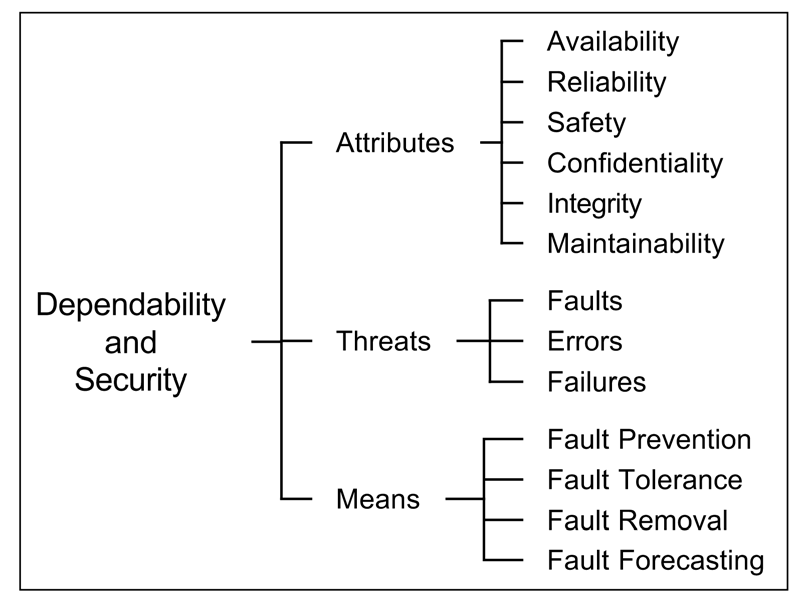
\includegraphics[width=0.65\textwidth]{figures/DepTax.PNG}
\caption{Dependability Taxonomy~\cite{art:Avizienis}}
\label{fig:deptax}
\end {figure}

The dependable system is a system, which has the ability to deliver it's service with acceptable number and severity of system failures~\cite{art:Avizienis}. Dependability ensures then the quality of the system's service~\cite{art:Laprie}. Above all the dependability is an integrating term that encapsulates following \textbf{attributes}:
\begin{itemize}
\item \textbf{availability} - readiness for the delivery of correct service, can be used as a  measure, being a time function $A(t)$ showing the probability that the system functions correctly at the particular time $t$. 
\item \textbf{reliability} - permanence in the delivery of correct service, can also be used as a measure, being the time function $R(t)$ showing the probability that the system has functioned correctly in the time interval $[t_0,t]$ under assumption that it has functioned correctly at the time $t_0$.
\item \textbf{safety} - absence of catastrophic system failures and ability to transit and reside in the fail-safe state, again a measure being a time function $S(t)$ showing probability that a system that worked correctly at time $t_0$ works correctly in the interval $[t_0,t]$ or remains in the fail-safe state,
\item \textbf{maintainability} - possibility of the system alteration and repairs (by authorized subjects) given as a time function $M(t)$ showing the probability that a faulty system will be repaired within time $t$~\cite{art:Laprie, art:Avizienis}.
\end{itemize}
The mentioned above definitions are based on two important terms: system failure and correct service, being in fact antonyms. The absence of one means the presence of the other. A system failure is therefore one of the impairments that threaten the dependability. There are three \textbf{threats}, that form a hierarchical structure:
\begin{itemize}
    \item \textbf{failure} - a state when system delivers service that deviates from the functional specification or the specification describes systems function not adequately; also a transition from a correct state to the described state. Failure happens as a consequence of an error.
    \item \textbf{error} - part of the system state, which may lead to the system failure, but doesn't have to. An error may be latent (after the fault occurrence) or get activated and become effective,
    \item \textbf{fault} - a primary term, an undesired circumstance affecting the system, being a cause of an error~\cite{art:Avizienis}. 
\end{itemize}
An example seems appropriate to illustrate the differences and relationship between dependability threats. \\
Let's consider a short-circuit within an integrated circuit and call it a fault. The result of the short, being one of the connections stuck at a boolean value - an error. The error remains latent until it doesn't get activated. In this scenario the activation would be an attempt of a logical switch of this connection to the opposite value, causing a failure of the connection - an obvious deviation from the specified behavior (reproduction of the input signal to the output of the connection). But a failure of one connection doesn't [have to] mean a failure of the whole integrated circuit. The hierarchical structure of dependability threats and a general hierarchical structure of systems results in the cause and effect relationship called error propagation. It is illustrated in the {Figure~\ref*{fig:propagation}}. An error gets internally propagated until it reaches the interface of another systems component. The failure of one component creates an error in the interfaced component. If this error leads to incorrect service of the entire system, then it means the system failure occurred~\cite{art:Avizienis}. \\

\begin  {figure}  [H]
\centering
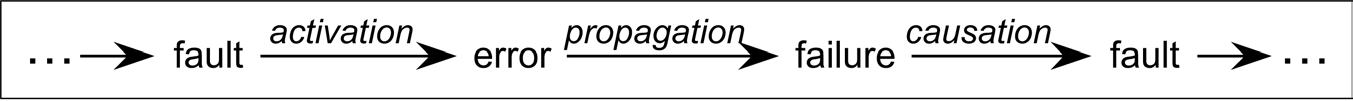
\includegraphics[width=0.65\textwidth]{figures/propagation.png}
\caption{The chain of dependability~\cite{art:Avizienis}}
\label{fig:propagation}
\end {figure}

Knowing what the dependability is and what are the threats it is important to know what available \textbf{means} do developer have to create a dependable system. There are four solutions:
\begin{itemize}
    \item \textbf{Fault Prevention} aims mostly at the development phase of a system and relays on design rules, modularization and strongly-typed languages. It also records the detected faults and eliminates them through development process modification.
    \item \textbf{Fault Tolerance} stands for methods which imply the presence of faults and their inevitability. Hence the need for error detection and processing. The fault tolerance is elaborated in the {section~\ref*{sec:tolerance}}.
    \item \textbf{Fault Removal} in the development phase has three stages: verification, diagnosis and correction. If the verification shows faults in the system, the two other steps need to by applied. The verification needs to be repeated afterwards. In the use phase the faults are removed through maintenance, which requires an external agent (a repairman, some test equipment or software).
    \item \textbf{Fault Forecasting} bases on evaluation process of the system behavior, especially the fault occurrence and activation. The evaluation can be either qualitative - classify and rank events that are dangerous to the system; or quantitative - count and give probabilistic measure of the extent in which the attributes of dependability are satisfied. 
\end{itemize}
While the fault prevention and the fault forecasting are more useful in analysis of the system dependability and aim to minimize the amount and severity of faults in the system, thus helping by the fault avoidance; the fault tolerance and fault removal both assume that the faults happen and provide methods to reduce their impact on the system, creating a group of fault acceptance methods, thus helping by handling with systems that are subject to faults. {Figure~\ref*{fig:depgroup}} represents the grouping of dependability means.

\begin  {figure}  [H]
\centering
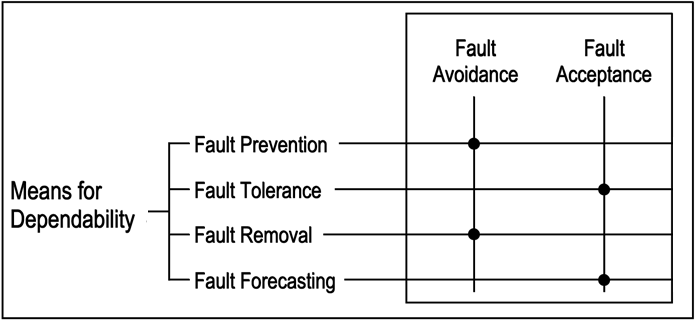
\includegraphics[width=0.65\textwidth]{figures/depgroup.png}
\caption{Grouping of the means for dependability~\cite{art:Avizienis}}
\label{fig:depgroup}
\end {figure}
\section{Fault taxonomy}
There are eight categories that help to understand what kinds of faults there are and how they may influence the system. They are called the elementary fault classes. Each fault falls into more classes. They may be understood as properties of a fault. The possible combinations are marked with a dot in the~{Figure~\ref*{fig:fault}}. The developer has to decide witch classes should be included in the dependability specification 

\begin  {figure}  [H]
\centering
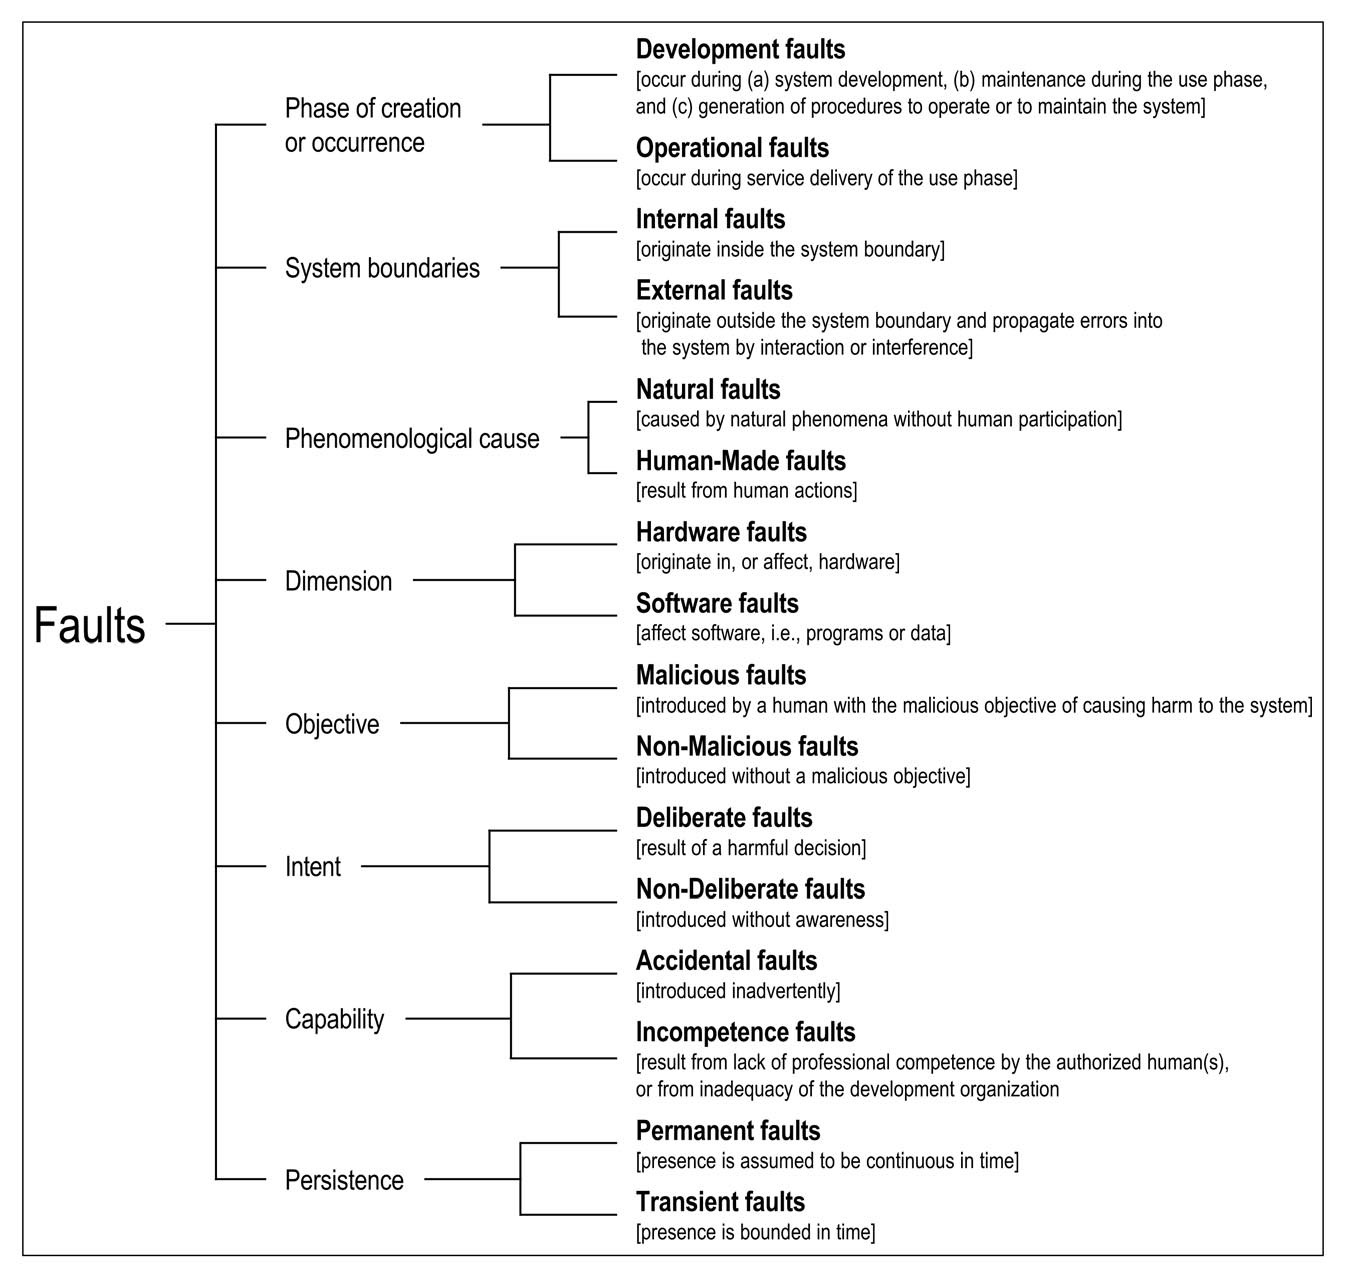
\includegraphics[width=0.65\textwidth]{figures/fault.png}
\caption{The elementary fault classes~\cite{art:Avizienis}}
\label{fig:fault}
\end {figure}

The classes divide into three main groups: the development faults, the physical faults and the interaction faults. The development faults occur during the development phase of the system, they partially overlap with the physical faults, which are all the faults that affect the hardware. The last group describes faults that happen during the use phase and come from the use environment of the system, hence they are operational faults.\\
Very important perspective splits faults up into two, or actually three groups, based on the duration of the fault and its persistence:
\begin{itemize}
    \item The \textbf{transient faults} occur once and don't persist afterwards. The error caused by such a fault is called a soft error.
    \item The \textbf{permanent faults}, often called hard faults, occur at some point in time and last until the faulty component gets repaired. Faults occurrence may happen already in the development phase and results in erroneous data being produced by affected component during its use. 
    \item The \textbf{intermittent faults} occur repeatedly but not continuously in the same spot in the design. The errors caused by such faults tend to also be intermittent~\cite{book:Sorin}.
\end{itemize}
The knowledge about the faults persistence is therefore important, that it changes the strategy of fault tolerance. The permanent faults, to be removed, require some sort of repair procedure, while the transient faults require much less complicated treatment, like repetition of the operation.


%definition and taxonomy.  Distinguish faults errors and failures. Permanent and transient faults, wireless strongly disturbed medium, radiation, hardware faults. Means of Dependability, Fault tolerance against fault avoidance
\section{Fault Tolerance}


\section{Channel Coding} \label{sec:cod}
In the year 1948 Shannon published a landmarking paper "Mathematical Theory of Communication" where he showed that, with a certain information encoding, the errors induced by a noisy channel can be reduced to any suitable level~\cite{art:Shannon}. With this article he started the era of coding theory and a race to create better and better codes with simple decoding algorithms~\cite{book:Lint}. He laid the mathematical foundation of reliable communication, which gets improved until this day.\\

\begin  {figure}  [H]
\centering
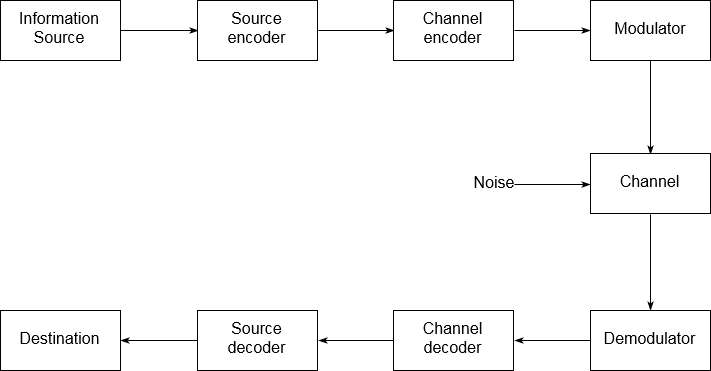
\includegraphics[width=0.65\textwidth]{figures/Data_transmission_path.png}
\caption{Block diagram of a typical data transmission (storage) system~\cite{book:LinCostello}}
\label{fig:data_path}
\end {figure}

\noindent\hyperref[fig:data_path]{Figure~\ref*{fig:data_path}} represents a typical information transmission system. Firstly the source encoder transforms the source output into a sequence of bits, called \textit{information sequence} \textbf{u}, trying to minimize the number of bits needed to represent the source output. The source output should be easily reproduced by the source decoder without ambiguity. The purpose of the channel encoder is to transform the information sequence into a discrete sequence \textbf{v} called the \textit{code~word}. The code word should allow the channel decoder, despite possible errors, to reproduce the information sequence. Since the discrete symbols are not applicable for transmission they need to be translated into the waveform and then sent to the receiver, that's why the channel encoder is followed by the modulator. The received, possibly disturbed signal has to be demodulated into a discrete \textit{received sequence}~\textbf{r}. The channel decoder uses the received sequence to reconstruct the code word and in result, hopefully error-free, \textit{estimated~sequence~\textbf{\^{u}}}; which in the perfect scenario is equal to the information sequence, produced by the source encoder. The very last stage is to transform the information sequence into the destination input, which should by absolutely equal to the source output~\cite{book:LinCostello}.\\

\section{Redundancy} \label{sec:red}
There are many arts of redundancy 
The additional information added by the encoder is called the \textit{redundancy} and it's a necessary element for error detection which can further lead to error correction. There are two main approaches to error correction.\\[\baselineskip]
\textbf{Error Correction Through Retransmission} is based on an assumption, that after the detection of an error, there is enough time to retransmit the code word. The redundancy results in the additional control bits for error detection and in the additional time for retransmission. The codes used in this approach are called Error Detecting Codes (EDC)\\[\baselineskip]
\textbf{Forward Error Correction} enables localization of the error position in the code word and as a result, reconstruction of the original code word and information sequence, without the need of the code word retransmission. The only redundancy are the control bits. The codes used in this approach are called Error Correcting Codes (ECC)~\cite{book:SchonfeldKlimant}.\\

\subsection{Code Redundancy}\label{sub:red}

There are two main groups of codes, block codes and convolutional codes. Since the convolutional codes are not used in the ParSec Project, the understanding of their creation and properties is negligible for the sake of this thesis, therefor a redirection to~\cite{book:Lint}(Chapter 11) seems appropriate.
The block codes


%=============================================================
% All appendices and extra material, if you have any.
\cleardoublepage
\appendix%

%\chapter{Rysunki techniczne}
\begin{figure} [h]
\centering
%%----start of first subfigure----
	\subfloat[G�rna warstwa p�ytki]{\label{fig:subfig:front} 
	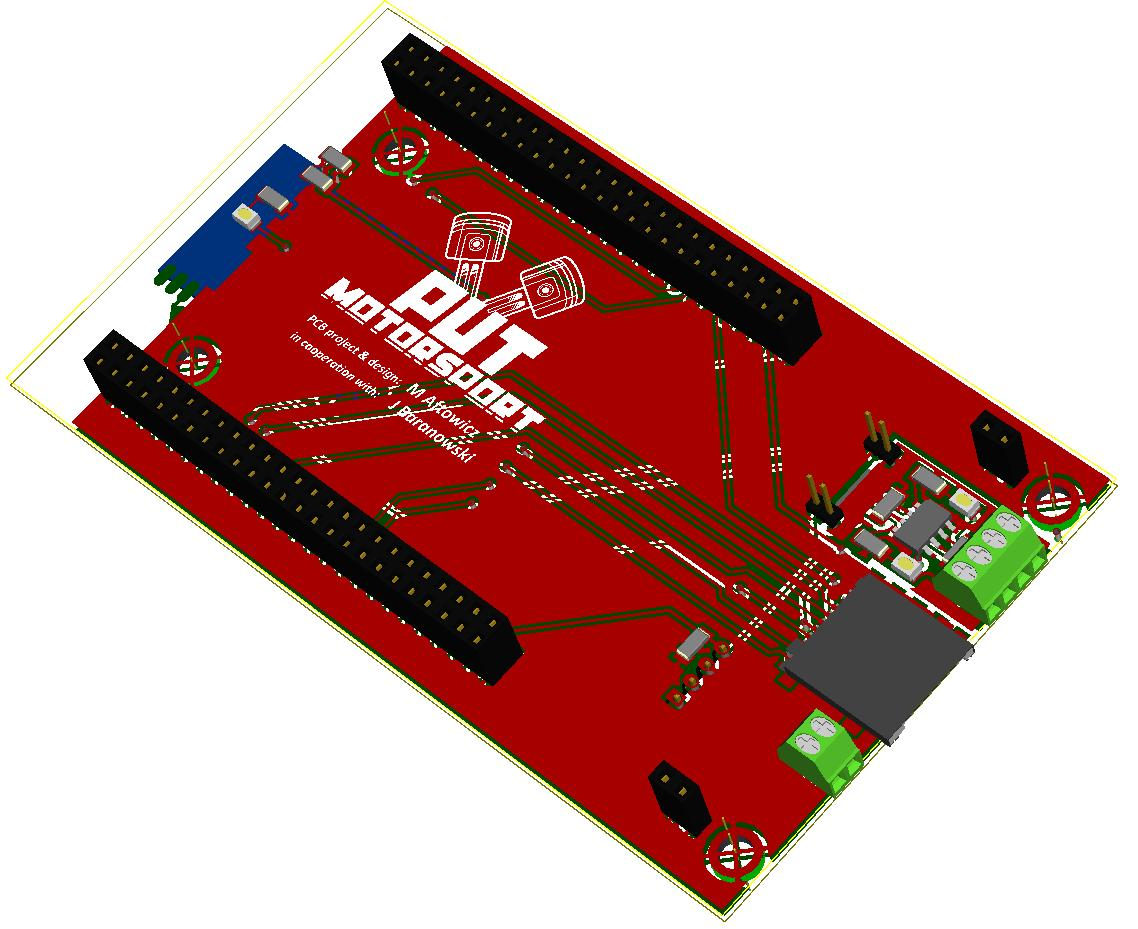
\includegraphics[height=0.3\textheight]{figures/Board_PCB_front.JPG}}
	\hfill
%%----start of second subfigure----
	\subfloat[Dolna warstwa p�ytki]{\label{fig:subfig:back}
	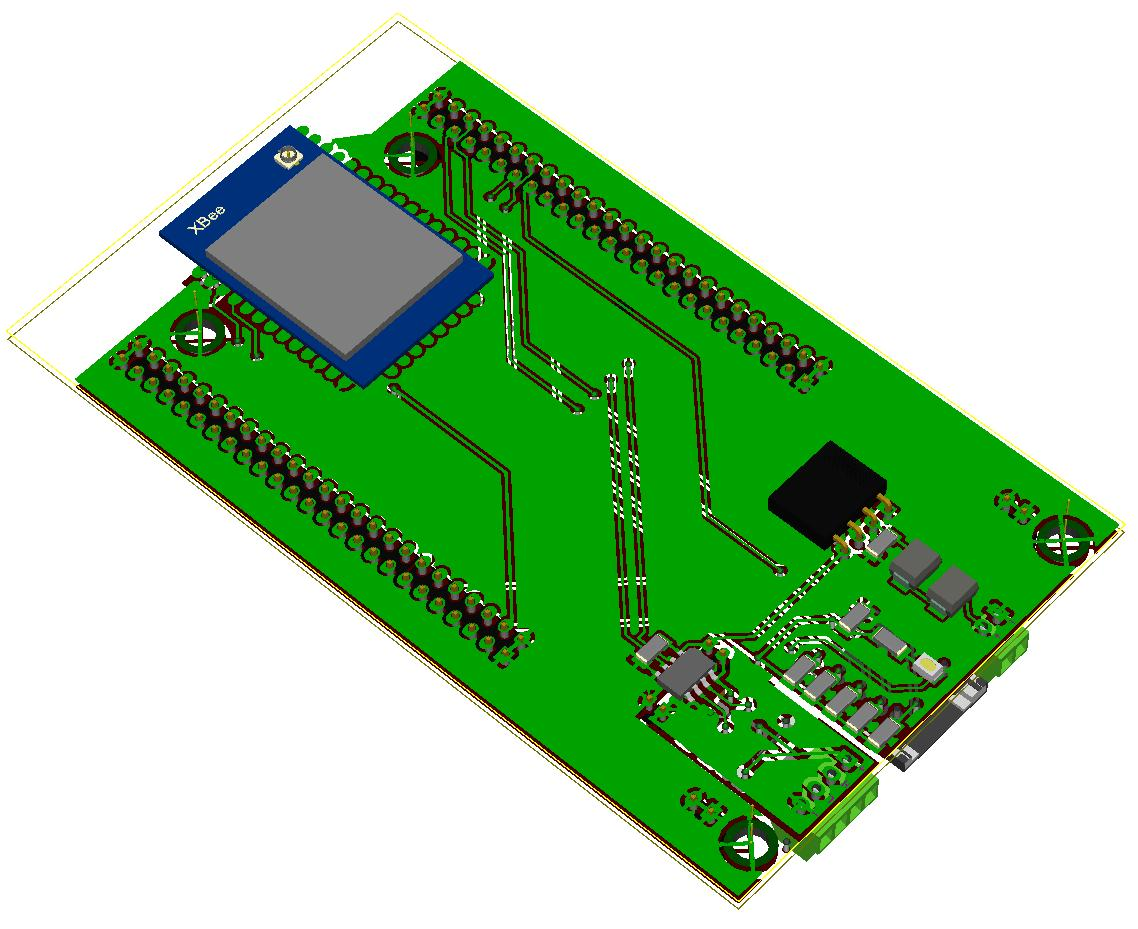
\includegraphics[height=0.3\textheight]{figures/Board_PCB_back.JPG}}
	\caption{Model 3D nak�adki na Discovery}
	\label{fig:3D} %% label for entire figure
\end{figure}

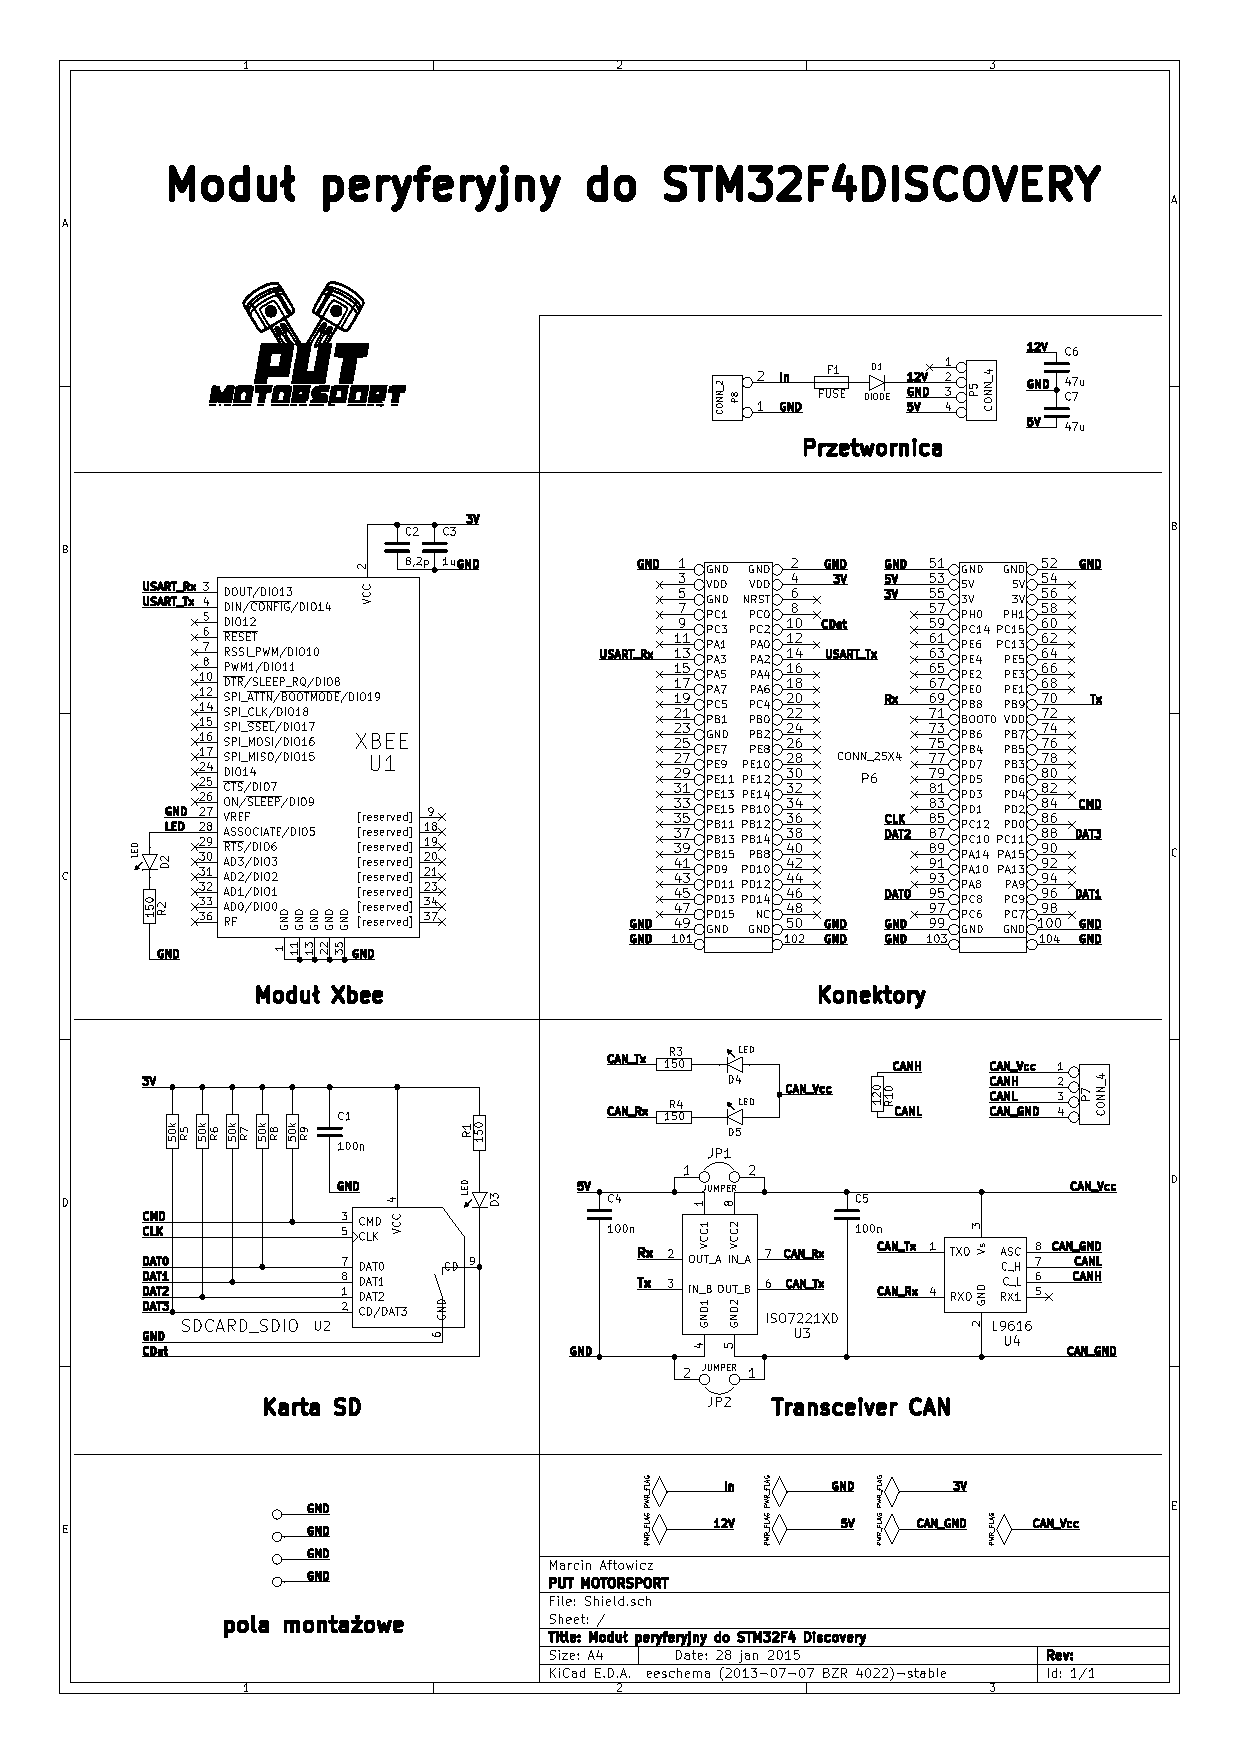
\includepdf[trim=0 0 -1cm 0, pages={1}]{figures/Motherboard_bw.pdf}
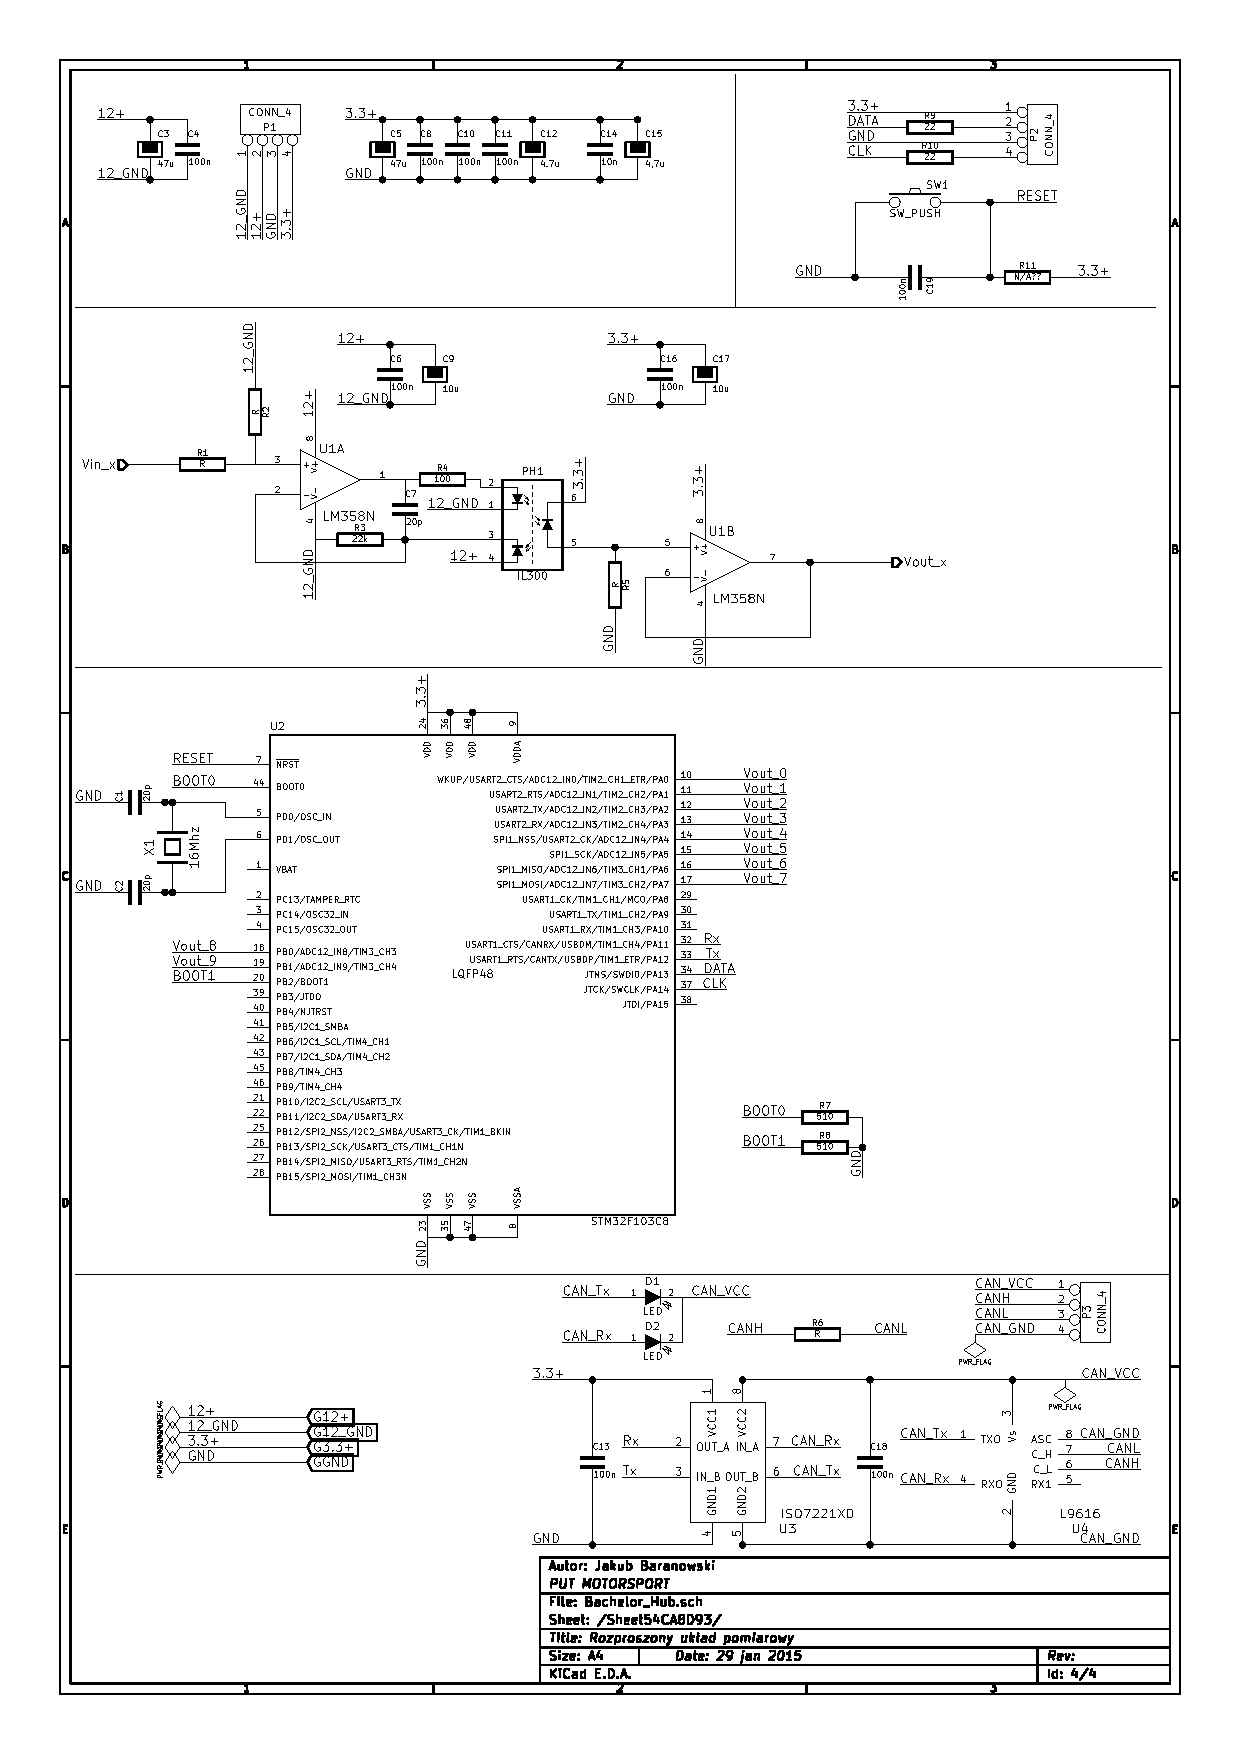
\includepdf[trim=-1cm 0 0 0, pages={1}]{figures/Bachelor_Hub.pdf}
\noindent



%%\input{plyta.tex}
%\cleardoublepage
\hypersetup{ linkcolor={black}}
\cleardoublepage

\bibliography{bibliografia}
\end{document}